\documentclass[12pt]{article}
\usepackage{amsmath}
\usepackage{amssymb}
\usepackage{geometry}
\usepackage{graphicx}

\geometry{a4paper, margin=1in}

\title{CSE 3504: Homework 6}
\author{Isaac Piegat}
\date{11/27/2024}

\begin{document}

\maketitle

\section*{Problem 1:}

\subsection*{1a.}

\begin{center}
    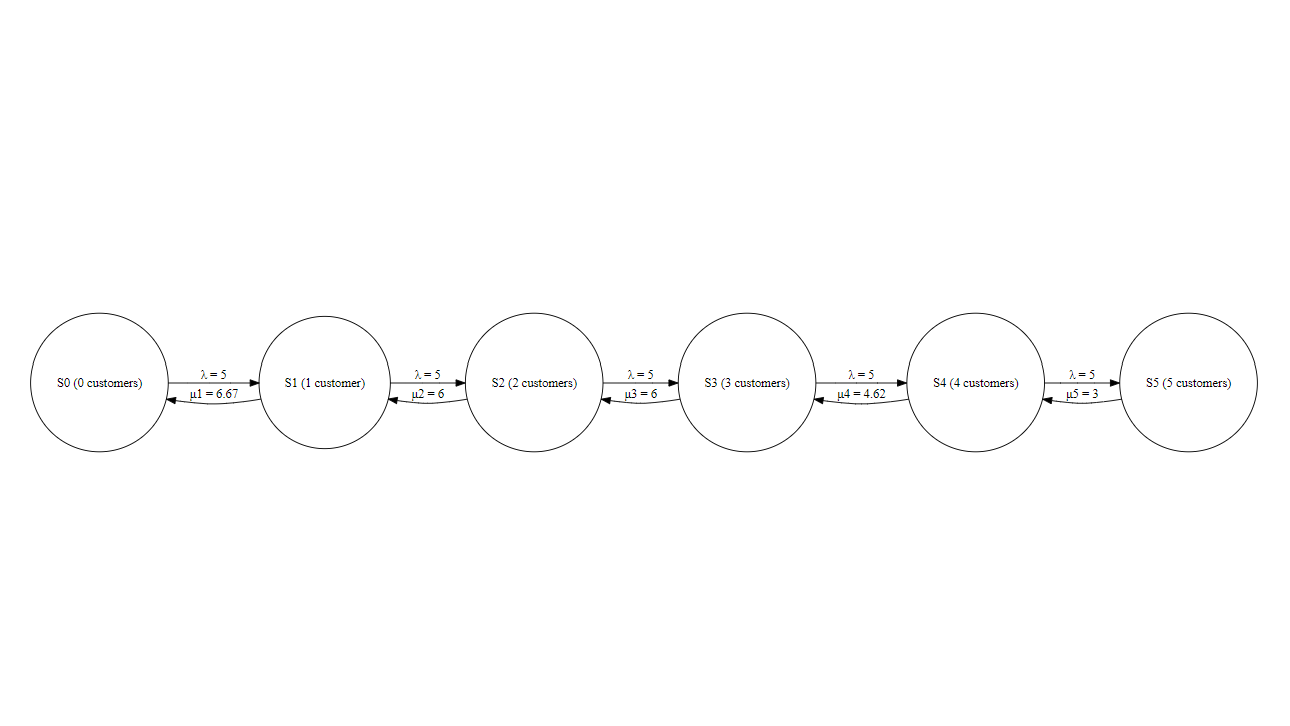
\includegraphics[width=0.8\textwidth]{state_transition_diagram.png}
\end{center}

\subsection*{1b.}

\[
\lambda P_0 = \mu_1 P_1
\]

\[
(\lambda + \mu_1)P_1 = \lambda P_0 + \mu_2 P_2
\]

\[
(\lambda + \mu_2)P_2 = \lambda P_1 + \mu_3 P_3
\]

\[
(\lambda + \mu_3)P_3 = \lambda P_2 + \mu_4 P_4
\]

\[
(\lambda + \mu_4)P_4 = \lambda P_3 + \mu_5 P_5
\]

\[
\mu_5 P_5 = \lambda P_4
\]

\[
P_0 + P_1 + P_2 + P_3 + P_4 + P_5 = 1
\]

\subsection*{1c.}
\[
Q =
\begin{bmatrix}
-5 & 5 & 0 & 0 & 0 & 0 \\
6.67 & -11.67 & 5 & 0 & 0 & 0 \\
0 & 6 & -11 & 5 & 0 & 0 \\
0 & 0 & 6 & -11 & 5 & 0 \\
0 & 0 & 0 & 4.62 & -9.62 & 5 \\
0 & 0 & 0 & 0 & 3 & -3
\end{bmatrix}
\]

\subsection*{1d.}

\begin{verbatim}
lambda <- 5
mu <- c(6.67, 6, 6, 4.62, 3)

P0 <- 1 / (1 + lambda/mu[1] + (lambda^2)/(mu[1]*mu[2]) + (lambda^3)/(mu[1]*mu[2]*mu[3]) + 
           (lambda^4)/(mu[1]*mu[2]*mu[3]*mu[4]) + (lambda^5)/(mu[1]*mu[2]*mu[3]*mu[4]*mu[5]))

P <- numeric(6)
P[1] <- P0
for (i in 2:6) {
  P[i] <- P[i-1] * lambda / mu[i-1]
}

P_idle <- P[1]         
P_reject <- P[6]       
L <- sum((0:5) * P)    

cat("Probability the hairstylist is idle:", P_idle, "\n")
cat("Probability an incoming request is turned away:", P_reject, "\n")
cat("Average number of customers in the system:", L, "\n")
\end{verbatim}

\textbf{Results:}
\begin{itemize}
    \item \(P_0 = \text{0.2274143 }\)
    \item \(P_5 = \text{0.2135385}\)
    \item \(L = \text{2.389943}\)
\end{itemize}

\section*{Problem 2:}

\subsection*{2a.}
\[
\rho = \frac{\lambda}{\mu} = \frac{20}{30} = 0.6667
\]
\[
\rho = 0.6667 \, \text{(or 66.67\%)}
\]

\subsection*{2b.}
\[
L = \frac{\rho}{1 - \rho} = \frac{0.6667}{1 - 0.6667} = 2
\]

\subsection*{2c.}
\[
L_q = \rho \cdot L = 0.6667 \cdot 2 = 1.3334
\]

\subsection*{2d.}
\[
W = \frac{L}{\lambda} = \frac{2}{20} = 0.1 \, \text{hours} = 6 \, \text{minutes}
\]

\subsection*{2e.}
\[
W_q = \frac{L_q}{\lambda} = \frac{1.3334}{20} = 0.06667 \, \text{hours} = 4 \, \text{minutes}
\]

\subsection*{2f.}
\[
P_{n \geq 5} = \rho^5 = 0.6667^5 \approx 0.1317
\]

\section*{Problem 3:}

\subsection*{3a.}
\[
L = \sum_{n=0}^{4} n \cdot p_n = (0 \cdot \frac{1}{6}) + (1 \cdot \frac{4}{16}) + (2 \cdot \frac{6}{16}) + (3 \cdot \frac{4}{16}) + (4 \cdot \frac{1}{16}) = 2
\]
\[
L = 2
\]

\subsection*{3b.}
\[
\text{Customers served} = (1 \cdot \frac{4}{16}) + (2 \cdot \frac{6}{16}) + (2 \cdot \frac{4}{16}) + (2 \cdot \frac{1}{16}) = 1.625
\]
\[
L_q = L - \text{Customers served} = 2 - 1.625 = 0.375
\]

\[
L_q = 0.375
\]

\subsection*{3c.}
\[
\text{Customers served} = 1.625
\]

\subsection*{3d.}
\[
W = \frac{L}{\lambda} = \frac{2}{2} = 1 \, \text{hour}
\]
\[
W_q = \frac{L_q}{\lambda} = \frac{0.375}{2} = 0.1875 \, \text{hours} = 11.25 \, \text{minutes}
\]
\[
W = 1 \, \text{hour}
\]
\[
W_q = 11.25 \, \text{minutes}
\]

\subsection*{3e.}
\[
\text{Service Time} = W - W_q = 1 - 0.1875 = 0.8125 \, \text{hours} = 48.75 \, \text{minutes}
\]
\[
\text{Service Time} = 48.75 \, \text{minutes}
\]

\end{document}
